\section{Concept}

\subsection{Architecture}
    The overall architecture is the same as for the previous version. The survey tool
    uses a classical client-server approach, where the client is a 
    javascript application running inside a web browser. This approach
    enables everyone with a modern web browser to use the platform without
    having to install any additional software locally. Notable exceptions
    are Internet Explorer, Opera Mini and the Blackberry Browser, as they
    do not support the CSS \inline{grid} property fully.
    The server-side software stack is deployed by using docker and 
    exposed through a containerized web server.
    Communication between different containers on the server takes place
    on a virtual network which is not exposed to the internet. Communication
    between client and server is handled by a RESTful API which is provided
    by the server.

\subsection{Survey Content}
    During refactoring, the top-level organisational unit ``survey'' was removed
    and replaced by ``questionnaire''. Grouping multiple questionnaires
    inside a single survey only makes sense in a small set of use cases.
    For other use cases, this has proven to be confusing to users. Most of the time, 
    a survey contains only a single questionnaire. Use cases, where
    grouping of multiple questionnaires into a single survey is appropriate
    can still be achieved by creating multiple questionnaires without any
    explicit grouping. Apart from that, the overall survey structure did not
    change significantly.

    \subsubsection{Questionnaire}
        \begin{wrapfigure}{o}{.45\textwidth}
            \centering
            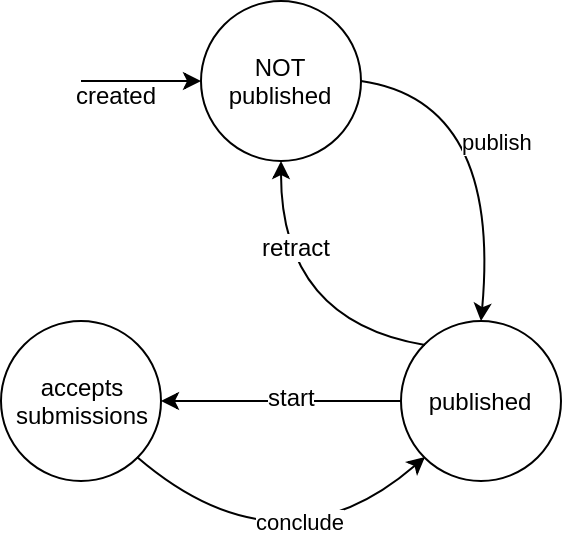
\includegraphics[width=.4\textwidth]{survey_lifecycle}
            \caption{Questionnaire life-cycle}
            \label{fig:survey-lifecycle}
        \end{wrapfigure}
        A questionnaire is a collection of dimensions, which also contains administrative
        information. A questionnaire's life cycle is modeled using three
        distinct states. The questionnaire starts out as not published,
        which means that it is only accessible to it's owner via the API
        (with the exception of templates, which will be accessible to other
        authenticated data clients)
        and will not display when accessed by data subjects via it's
        public URL. This state is meant for questionnaires which are
        incomplete and worked on. Once a questionnaire reaches it's
        published state, it will be visible to the public via it's
        public URL. It will not accept submissions via the API at this point.
        The publicly accessible representation of the questionnaire will
        not display form controls to submit and display an information
        page before accessing the survey content. This page informs the data subject,
        that submissions are not accepted at this point. Once data subjects
        are allowed to submit answers, the questionnaire enters
        the ``accepts submissions'' state. The public page will now display
        form controls to submit and new submissions are accepted by the API.
        Once the survey has concluded, the questionnaire returns to
        the ``published'' state and can be viewed for future reference.
        If this is not wanted, the data client has the option to retract
        the survey and return it to it's ``NOT published'' state.
        This life-cycle model is illustrated in figure \ref{fig:survey-lifecycle}.

        Along with information about it's life cycle, the questionnaire
        also stores information about any access control challenges
        presented to data subjects. As in the previous version, challenges
        are presented as additional form inputs when submitting. 
        In contrast to the previous version, email addresses are now always
        validated when submitting by sending a one-time-use token to the
        entered email address.
        Data clients may choose from these challenges:
        
        \begin{description}
            \item[Password:] A password has to be entered in order to submit.
            The password is chosen by the data client.
            \item[Email whitelist:] Only emails that are present in a list
            of email addresses are allowed to submit. The email whitelist
            also supports wildcard expressions to allow all email addresses
            following a certain schema.
            \item[Email blacklist:] The same as email whitelist, but instead
            of allowing certain email addresses, this blocks certain addresses
            from participating.
        \end{description}
        
    \subsubsection{Dimension}
        A dimension is a collection of questions usually pertaining to
        a specific topic. The only additional piece of information
        handled by the dimension is whether the order of it's questions
        should be randomized when the survey is taken.

    \subsubsection{Question}
        A question is a single statement to which the data subject may respond
        on a numerical scale. Lower and upper bounds of this scale
        may be adjusted by the data client, as well as the descriptions
        for these bounds. Individual questions may be used as templates,
        which is why the information on lower and upper bounds and scale
        labels is stored on a per-question basis. Convenience workflows
        for updating this information for an entire dimension allow
        easy editing despite the great granularity of this approach.

\subsection{Internationalisation}
    Every time an API request is made,
    a request language is determined by the server and the request is
    handled in this language.
    For human readable attributes of survey items, multiple translations
    may exist. When a survey item is created, the language it is created
    in becomes the item's original language. Translations in different
    languages may be added later by updating the survey item using 
    the desired language as the request language. 
    When no translations for the requested language exist, survey items 
    are served in their original language instead.
    To communicate information about existing translations and
    what translation was served, the API includes the item's
    current language, original language and a list of available languages
    in the JSON representation of the item.

\subsection{Ownership, Parties, Roles}
    To control API access to survey items, survey items had a single
    owner in the previous version. Owner refers to a data client who has access
    to the resource. In the next version, the ownership model
    was expanded to allow n-to-n relationships between owning parties
    and owned resources. Ownership is also no longer restricted to
    data clients. These changes became necessary for two reasons.
    Survey item are no longer the only resource with access restrictions,
    as will become clear in section \ref{sec:modification-tracking}.
    While survey items ususally only have a single owner - the author - 
    tracking information has to be accessible to all parties sharing
    read access to the tracked resource. Because of the template management,
    data clients may have read access to survey items of which they're not
    the author (templates). This requires a single resource to have multiple owners.
    Of course, a party may own more than a single resource, hence the n to n
    cardinality of this relationship. The reason for expanding ownership
    to data subjects is that the mechanism makes it easy to identify personal
    data. Data subjects own all resources which contain
    personal data. The ``right to be forgotten'' may then be implemented by
    simpy retrieving all owned objects for a given data subject and deleting 
    them from the database.

    For some priviliged users, access control should not be enforced.
    Also, the right to publish templates is reserved for a select
    group of users. To accomplish different levels of privilege,
    roles were introduced to all parties. A party may have a number
    of different roles, depending on the actions they may take and
    the data they may access. There are currently five different roles:

    \begin{table}[H]
        \begin{tabularx}{\textwidth}{|l|l|X|}
            \hline
            Role & ID & Description \\
            \hline \hline
            Root & 0 & All available access control methods grant access to users with this role. \\
            Admin & 10 & An administrative user, who may view and modify other user's data in order to ensure proper operation of the platform. \\
            Contributor & 20 & A user who may make survey items available to other users as templates. \\
            User & 30 & A regular user who may create and modify their own survey items. \\
            Unprivileged & 40 & A user who may view and participate in published surveys, but not create or modify survey items. This role is used for all data subjects.\\
            \hline
        \end{tabularx}
    \end{table}

    Access control may then be enforced by checking if the role required
    for a certain action is held by the user in question.

\subsection{Modification Tracking}
\label{section:modification-tracking}
    To track modifications of survey items, every time a modification
    is made to an item, a record of this modification is stored in the
    database. To keep storage space needed for this feature to a minimum,
    only the most recent modification for each attribute is stored.
    During development it was discovered that different kinds of modifications
    require different information to be stored in order to create a meaningful
    record of the change, which can also be presented to the data client.
    Such information includes: The modified item, the modifying data client,
    previous and new values, as well as the point in time when the modification
    occurred. Five different types of records were identified:

    \begin{table}[H]
        \begin{tabularx}{\textwidth}{|l|l|X|}
            \hline
            \# & Description & Stored information \\
            \hline \hline
            1 & An attribute was updated  & Modified item, modifying data client, attribute name, previous value, new value, timestamp \\
            2 & A language map was updated & Modified item, modifying data client, attribute name, modified language name, previous value, new value, timestamp \\
            \hline
            3 & A child item was added & Parent item, modifying data client, child item, timestamp \\
            4 & A child item was removed & Parent item, modifying data client, child item name, timestamp \\
            \hline
            5 & A questionnaire was removed & Name of the questionnaire, modifying data client, timestamp\\
            \hline
        \end{tabularx}
    \end{table}

    The modified item is stored as a reference to the actual record of the item in the database.
    This makes it possible to quickly find the modified item based on
    a tracking record. In the user interface, this is used to display the
    modified item as a clickable link, which will show the modified item
    instantly. For types of modifications, where an item was deleted, this 
    kind of data model is not applicable, as the referenced record won't 
    exist in the database anymore. In these instances, only the name of
    the item is stored. A special case exists for the deletion of questionnaires,
    as they don't have parent item needed to construct the tracking record.
    In this case, only the questionnaire name is stored.
    To deliver a personalized stream of modifications to data clients,
    including only those modifications which are of interest to them,
    tracking records also use the ownership model.
    Tracking recors are owned by all parties interested in the tracked
    item.

\subsection{Template Management}
    A template refers to a survey item, from which other survey items
    ay be created as copies. A copy of a template should always
    mirror the template's content, including it's relationships
    to it's children, as the children are part of the item's content.
    This is true, since all parent-child relationships 
    of survey items are aggregations; a dimension has no purpose
    without any questions and a questionnaire has no purpose
    without any dimensions. Every survey item may optionally also
    be a template. Survey items may be made available as a template by 
    any data client who has at least the \inline{Contributor} role.
    Templates are visible to all data clients.


\subsection{xAPI Support}
    \subsubsection{Introduction to xAPI}
        xAPI, formerly known as TinCanAPI, is a data exchange
        standard closely resembling activity streams \cite{activity-streams}.
        It was developed by the Advanced Distributed Learning (ADL) Intiative
        as a successor to SCORM \cite{scorm,xapi-history} and allows the exchange of experiential
        information in the form of statements \cite{xapi-object-model}. These statements
        use JSON as their data format and include a minimum of three
        semantical objects, ``actor'', ``verb'' and ``object''. 
        The data is transmitted using HTTP, following REST principles.

        \begin{figure}[H]
            \begin{lstlisting}[language=JSON]
{
    "actor": {...},
    "context": {
        "contextActivities": {
            "grouping": [
                {...}
            ],
            "parent": [
                {...}
            ]
        },
        "extensions": {
            "http://activitystrea.ms/schema/1.0/place": {...}
        },
        "language": "en",
        "platform": "st3k101 via localhost"
    },
    "id": "896ef7f1-8d5c-4729-b028-e9d72df47fe8",
    "object": {...},
    "result": [
        {...}
    ],
    "timestamp": "2018-09-27T14:32:15.009513",
    "verb": {...}
}

            \end{lstlisting}
            \caption{Anatomy of an xAPI statement}
            \label{fig:anatomy-xapi-statement}
        \end{figure}
    
    An xAPI statement may also include a ``timestamp'' stating the
    issue date and time of the statement, a ``context'', providing
    additional information about the event and a ``result'', detailing
    the outcome or outcomes of the event. The format is also extensible,
    additional information can be provided in the ``extensions''
    object inside the ``context''.

\subsubsection{xAPI Statement Design}
    There are several actions which will trigger sending of an
    xAPI statement:

    \begin{figure}[H]
        \begin{itemize}
            \item[1)] A data client logs in into the survey platform.
            \item[2)] A data subject launches an embedded survey.
            \item[3)] A data subject answers a single question.
            \item[4)] A data subject answers a known survey item (whole questionnaire or dimension)
            \item[5)] A data client updates the xAPI activity ID of a survey item.
        \end{itemize}
        \caption{List of cases where xAPI statements are emitted}
        \label{fig:xapi-statement-list}
    \end{figure}

    For each of these cases, an xAPI statement had to be designed.
    All of these statements share at least some of their structure.
    The \inline{context} object of all xAPI statements emitted by the survey
    tool includes the \inline{platform}, \inline{language} and 
    \inline{extensions} attributes. The \inline{language} attribute always
    contains an RFC 5646 \cite{rfc-5646}
    compliant representation of the language the action was performed
    in. The \inline{platform} attribute always starts with the
    string \inline{st3k101}, identifying the origin of the statement.
    The \inline{platform} attribute may also include the URL
    of the source LMS in the case LTI was used. In this case,
    the URL is appended as \inline{st3k101 via SOURCE_LMS_URL}.
    The \inline{extensions} object of the \inline{context} also
    includes a geolocation for the client in RFC 7946 compliant GeoJSON
    format \cite{rfc-7946}.
    Below is a concept for what additional data should be included in 
    the statements listed in \ref{fig:xapi-statement-list}.

    \begin{table}[h]
        \begin{tabularx}{\textwidth}{|l|l|l|X|X|X|}
            \hline
            \# & Actor & Verb & Object & Result & Context \\ 
            \hline \hline
            1 & data client & logged in & login page & - & - \\ 
            2 & data subject & accessed & questionnaire & - & - \\ 
            3 & data subject & answered & question & response value & parent dimension AND questionnaire  \\ 
            4 & data subject & answered & qestionnare OR dimension & response value & parent item, if any \\ 
            5 & data client & updated & questionnaire OR dimension OR question & new acitivity ID & - \\ 
            \hline
        \end{tabularx}
        \caption{Concept for information included in emitted xAPI statements}
        \label{table:xapi-data-concept}
    \end{table}

    Objects are identified by their \inline{objectType}, \inline{type} and \inline{id} in xAPI, 
    whereas verbs are just identified by their \inline{id}. For the purpose of the
    survey tool, all objects share the same \inline{objectType}, the \inline{Activity}.
    It is common practice to use a URL as identifier or type,
    which will return a human readable description of the item via HTTP GET. In theory,
    there's no correct identifier to use when designing xAPI statements, as the
    standard does not prescribe the use of any specific verbs or objects. In practice,
    several registries with commonly used verbs and objects exist and should
    be consulted when choosing which identifier or type to use. This avoids re-definitions
    of already existing items and increases homogeneity among statements by
    different adopters of the standard. Examples for these registries are \url{xapi.vocab.pub}
    and \url{registry.tincanapi.com}. The verbs and objects 
    used in table \ref{table:xapi-data-concept} had to be translated into already existing
    verbs and objects. The results are detailed in table \ref{table:xapi-identifiers-used}.
    For some of the objects, no suitable definitions existed. For those
    objects, dummy identifiers or types were used, which follow the URL format, but use 
    \inline{http://fantasy.land/} as a prefix.

    \begin{table}
        \begin{tabularx}{\textwidth}{|l|X|}
            \hline
            Verb & Identifier \\
            \hline 
            logged in & \url{https://brindlewaye.com/xAPITerms/verbs/loggedin} \\
            accessed & \url{https://w3id.org/xapi/dod-isd/verbs/accessed}\\
            answered & \url{http://adlnet.gov/expapi/verbs/answered}\\
            updated & \url{http://activitystrea.ms/schema/1.0/update}\\
            \hline \hline
            Object & Type \\
            \hline
            login page & \url{http://activitystrea.ms/schema/1.0/page}\\
            questionnaire & \url{http://id.tincanapi.com/activitytype/survey}\\
            dimension & \url{http://fantasy.land/dimension}\\
            question & \url{http://adlnet.gov/expapi/activities/question} \\
            \hline
        \end{tabularx}
        \caption{Used xAPI verb identifiers and object types}
        \label{table:xapi-identifiers-used}
    \end{table}

    In order to corellate objects in emitted xAPI statements with survey
    items in the survey tool, all survey items have a user-modifiable
    xAPI acitivity ID associated with them. This identifier is
    used as the object's \inline{id} in xAPI statements.
    These identifiers are not modifiable in copies of templates,
    which means that all instances of a copy will use the same xAPI
    activity ID. This is useful for conducting meta-analyses, where
    all results for a certain template could be included in the analysis,
    regardless of who conducted the survey. During testing, this
    presented itself as an issue, because results for the same template,
    which were collected by different data clients would not be distinguishable,
    as they all used the same identifier. For this reason,
    the email address of the data client who conducts the survey
    is added as a prefix to all xAPI activity IDs before sending.
    In figure \ref{fig:example-xapi-activity-dimension}, an example
    of how survey items will be represented in xAPI is given. 

    \begin{figure}
        \begin{lstlisting}[language=JSON]
"object": {
    "definition": {
        "description": {
            "en-US": "This is a particular scale of a survey, it usually contains multiple questions."
        },
        "name": {
            "de": "5. Anstrengung"
        },
        "type": "http://fantasy.land/dimension"
    },
    "id": "<bla@blubl.net>:lernstrategien_wild_schiefele--5_anstrengung",
    "objectType": "Activity"
}
        \end{lstlisting}
        \caption{Example of how a dimension is represented as an xAPI acitivity object}
        \label{fig:example-xapi-activity-dimension}
    \end{figure}

    Actors may be represented in four different ways using xAPI. 
    The identifying feature is either the person's email adress in the case
    of the \inline{mbox} and \inline{mbox-sha1sum} actor types, an account id 
    in combination with a URL where the account is located in the case of the 
    \inline{account} actor type
    or OpenID identitiy in the case of the \inline{openid} actor type.
    Data clients are represented as \inline{mbox} actor types, while data subjects may 
    be represented by as \inline{mbox-sha1sum} actor types
    or, in the embedded use-case, as an \inline{account} actor type using their
    LTI user identifier. The latter is necessary, because the email address might not be available
    though LTI. The LTI user ID is, contrary to prior suppositions, not
    useful for data analysis, as Moodle will use the user entities database ID.
    Moodle does however communicate a username via LTI, which for the specific Moodle instance
    at Goethe University is the same as the data subject's CAS ID.
    To retain compatibility with other LMSs while taking this finding into account,
    the username will take precedence over the LTI ID, if it's present in the LTI request.
    The LTI ID is also not globally unqiue, as there may be separate LMSs which
    use the same IDs for different users. For this reason, the LTI user ID is
    prefixed with the identifier of the source LMS, which is always present in LTI requests.

    The recipient of the statements is determined by the object which is acted upon. 
    This makes intuitive sense, as the person owning a certain survey item is the one interested in
    collecting data on it. All survey items are on the highest level
    organized into some questionnaire and there's no use-case for different
    data consumers for individual parts of the questionnaire. 
    For this reason, recipients are configured on a per-questionnaire basis.
    For objects which don't have an owner, for example the survey tool's login
    page, a default recipient is configured system-wide.
    To recover from failure in the case that an xAPI statement
    can not be transmitted over a prolonged period of time, the
    statement as well as the recipient and timestamp of the failure
    are logged to file and may then periodically be recovered.

\subsection{Support for LTI}
\label{section:concept:lti}
    The embedded user interface is launched by the LMS using the LTI protocol.
    To identify the source LMS, a random token, the consumer key,
    is generated in the back-end for every questionnaire. To
    embed a questionnaire within the course context, an LTI request
    with the correct combination of request URL and consumer
    key has to be made by the LMS.
    Information about the user is already present in the
    request body and is used to identify the data subject. 
    Since there's some time between LTI launch request
    and survey submission, user information
    has to be stored on the server for this period of time.
    To achieve this, the required data is stored in the data subject's account.
    If a data subject accesses the service through LTI for the first time, 
    a new account is provisioned for them.
    When launching the survey tool via LTI, a session is created
    for the data subject and a session token is embedded into
    the user interface. Actions by the data client in the
    embedded user interface will use the embedded session token
    for authentication with the API. This mechanism allows
    the API to identify the data subject on every subsequent
    request. A valid LTI request is treated as sufficient
    authentication for the data subject, as the source LMS already
    authenticated the user prior to them accessing the questionnaire.

\subsection{Email validation}
    When data subjects participate in a standalone survey,
    it is difficult to recognize repeated submission by the same
    person. Most features used for identification, for example the client's
    IP address or cookies present in the browser can easily be
    modified by the data subject. Even more
    advanced measures, like browser fingerprinting, are ultimately
    controlled by the client, as communication with the server
    is handled by a publicly available API. For this reason,
    a third party has to be involved in validating the user's identity.
    The survey tool achieves this validation through email.
    When submitting responses, the data subject has to enter their
    email address. At this point, the responses are stored on the server,
    but no xAPI statements have been emitted and the responses do not
    yet count towards the generated statistics. 
    A randomly generated token is embedded into a URL pointing back to the survey tool. 
    This URL is then sent to the submitted email address. 
    Once the data subject follows the URL, the server will associate the 
    token with the user's responses in order to validate them.
    After validation, the appropriate xAPI statements are emitted.

\subsection{Privacy Considerations}
    As mentioned in section \ref{section:concept:lti}, when a data subject participates
    in a survey, a user account is provisioned for them. Removal
    of this account and all associated personal data may be performed
    via the API when authenticated as an admin user.
    In order for the admin to know which account to communicate
    to the API, the API allows admin users to query for existing
    user accounts. Data removal is limited to admin users,
    as removal of accounts by data subjects themselves would require
    some sort of authentication mechanism for data subjects.
    When an email address is present for the data subject,
    authorization via email is a possible solution for this.
    In this scenario, the data subject would receive an email
    with a randomly generated token, which can be used to remove their personal
    data. If there's no email present for the data subject, for example
    when the account was provisioned using LTI, or if the data subject
    hasn't got access to their email account, this mechanism fails.
    Therefore, email as sole mechanism for data removal is not a viable
    option at the moment.
    